%\documentclass[hyperref={pdfstartview=Fit}]{beamer}
\documentclass[hyperref={pdfstartview=Fit,pdfpagemode=FullScreen}]{beamer}
\mode<presentation>%
{
  \usetheme{Warsaw}
  \setbeamercovered{transparent}
}
\usepackage[english]{babel}
\usepackage[utf8]{inputenc}
\usepackage{epstopdf}
\usepackage{lmodern}
\usepackage[T1]{fontenc}

\usepackage[lined, boxed]{algorithm2e}

\newcommand{\imsize}{}
\providecommand{\abs}[1]{\left\lvert#1\right\rvert}

\newlength{\widthtmp}
\newcommand{\getWidth}[1]{%
  \settowidth{\widthtmp}{#1}%
  \the\widthtmp%
}

% Delete this, if you do not want the table of contents to pop up at
% the beginning of each subsection:
% \AtBeginSubsection[]
% {
%   \begin{frame}<beamer>{Outline}
%     \tableofcontents[currentsection,currentsubsection]
%   \end{frame}
% }


% If you wish to uncover everything in a step-wise fashion, uncomment
% the following command:

%\beamerdefaultoverlayspecification{<+->}

\title[Advection equation and antidiffusion]%
{Antidiffusion techniques to refine the numerical solution of the advection equation}

\subtitle{Case study: Smolarkiewicz' iterative approach}

\author[Burger, Wolterink]%
{Gerhard Burger \and Jelmer Wolterink}

\institute[Utrecht University]%
{
  Scientific Computing\\
  Department of Mathematics\\
  Utrecht University
}

\date[31-Oct-2011] %
{Project presentations SOAC, 31 October 2011}

\subject{Advection equation and antidiffusion}

 \pgfdeclareimage[height=0.5cm]{university-logo}{UU_logo_fullcolor_uncoated_sol_left}
 \logo{\pgfuseimage{university-logo}}

\begin{document}

\begin{frame}
  \titlepage
\end{frame}

\begin{frame}{Outline}
  \tableofcontents
  % You might wish to add the option [pausesections]
\end{frame}

\section{The advection equation in climate modelling}
\subsection{Importance}

\begin{frame}

\begin{block}{Advection}
Transport mechanism of a \textbf{substance} by a \textit{fluid}, due to the fluid's \underline{motion} in a particular direction.
\end{block}

Examples in ocean, atmosphere and climate modelling

\begin{itemize}
   \item Transport of \textbf{trace gasses} by \textit{air} due to \underline{wind}
   \item Transport of \textbf{heat} by \textit{ocean water} due to \underline{currents}
   \item Transport of \textbf{ice} by \textit{ocean water} due to \underline{currents}
   \item Transport of \textbf{warm and moist air} over a colder surface by \textit{air} due to \underline{wind}: advection fog
\end{itemize}

\begin{figure}
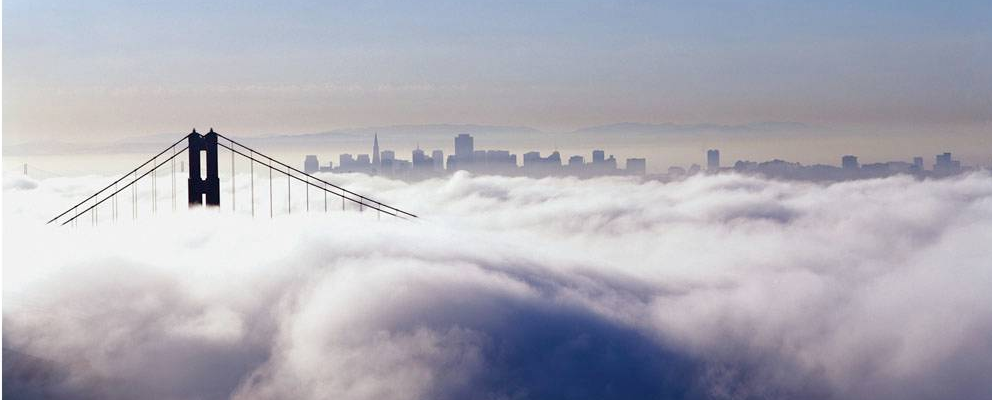
\includegraphics[width=7cm]{advfog.png}
\end{figure}

\end{frame}


\begin{frame}
\begin{block}{Advection equation}
Continuity equation describing the advection of a nondiffusive quantity in a flow field:

\begin{equation*}
\frac{\partial \psi}{\partial t} + \text{ div}(V\psi) = 0
\end{equation*}

where $\psi(x,y,z,t)$ is the nondiffusive scalar quantity, $V=(u,v,w)$ is the velocity vector and $x,y,z,t$ are the independent variables of space and time. 
\end{block}


\end{frame}

\begin{frame}
\frametitle{Advection simulation}

Constraints on advection simulation

\begin{itemize}
\item Solutions should contain no unphysical overshoot or undershoot: positive definite schemes
\item Methods should be volume preserving. No loss of matter
\item The solutions should be local: the solution at any one point should not be influenced by what is going on far away from that point
\end{itemize}

\end{frame}

\subsection{Diffusion}
\begin{frame}
\frametitle{Problem: diffusion}

\begin{itemize}
\item When simulating an advective process, we need to discretize space. When doing so, we introduce numerical constraints on the calculation and we get diffusion.
\item The numerical solution spreads out.
\item We get interactions, our simulations become less reliable.
\item $\Longrightarrow$ example
\end{itemize}

\end{frame}

\begin{frame}
\frametitle{Example of diffusion with an upstream scheme}
\begin{figure}
\renewcommand{\imsize}{0.7\textwidth}
\includegraphics<1>[width=\imsize]{animation/anime0}%
\includegraphics<2>[width=\imsize]{animation/anime1}%
\includegraphics<3>[width=\imsize]{animation/anime2}%
\includegraphics<4>[width=\imsize]{animation/anime3}%
\includegraphics<5>[width=\imsize]{animation/anime4}%
\includegraphics<6>[width=\imsize]{animation/anime5}%
\includegraphics<7>[width=\imsize]{animation/anime6}%
\includegraphics<8>[width=\imsize]{animation/anime7}%
\end{figure}
\end{frame}

\subsection{Antidiffusion methods}

\begin{frame}
\frametitle{Antidiffusion methods}
\begin{itemize}
\item Flux-corrected transport (FCT) method (Boris and Book, 1973),
\item self-adjusting hybrid scheme (SAHS) (Harten en Zwas, 1972),
\end{itemize}
   Both can be very accurate but require excessive computing time, better is the
\begin{itemize}
   \item hybrid-type scheme based on a Crowley advection scheme (Clark and Hall, 1979),
\end{itemize}
   with more diffusion but half the computation time.
\end{frame}

\begin{frame}
\frametitle{Antidiffusion methods}

\begin{block}{Smolarkiewicz' iterative correction, 1983}
\begin{itemize} 
\item Less time consuming while results are comparable to those of the more complex hybrid schemes
\item Positive semidefinite
\item Iterative method
\item Does not contain strong implicit diffusion
\end{itemize}
\end{block}
\end{frame}

\section{Case study: Smolarkiewicz}
\subsection{Analyzing the scheme}

\begin{frame}
1D case: $\frac{\partial \psi}{\partial t} + \frac{\partial}{\partial x}(u\psi) = 0$
\vspace{0.3cm}

\frametitle{Basis: upstream on a staggered grid}
We start with the following upstream advection equation on staggered grid:
\begin{equation*}
 \psi_i^{n+1} = \psi_i^n - \Big( F \left( \psi_i^n,\psi_{i+1}^n,u_{i+1/2}^n\right)
-F \left( \psi_{i-1}^n,\psi_{i}^n,u_{i-1/2}^n\right) \Big),
\end{equation*}
where
\begin{multline*}
F \left( \psi_i^n,\psi_{i+1}^n,u_{i+1/2}^n\right) =\\
\Big( \left( u_{i+1/2}^n + \abs{u_{i+1/2}^n} \right) \psi_i^n
+ \left( u_{i+1/2}^n - \abs{u_{i+1/2}^n} \right) \psi_{i+1}^n \Big)
\frac{\Delta t}{2 \Delta x}.
\end{multline*}
\end{frame}

\begin{frame}
\frametitle{Method of lines}
Writing the scheme out and collecting terms gives
\begin{equation*}
\begin{split}
\psi_i^{n+1} &=
\frac{\Delta t}{2 \Delta x} \left( u_{i-1/2}^n + \abs{u_{i-1/2}^n} \right) \psi_{i-1}^n\\
&+ \left(1 - \frac{\Delta t}{2 \Delta x} \left( u_{i+1/2}^n + \abs{u_{i+1/2}^n} - u_{i-1/2}^n + \abs{u_{i-1/2}^n} \right) \right) \psi_i^n\\
&-\frac{\Delta t}{2 \Delta x} \left( u_{i+1/2}^n - \abs{u_{i+1/2}^n} \right) \psi_{i+1}^n
\end{split}
\end{equation*}
\end{frame}

\begin{frame}
\frametitle{Method of lines}
This can be rewritten to 
\begin{equation*}
\psi_i^{n+1} = \alpha_i \psi_{i-1}^n + \beta_i \psi_i^n +\gamma_i \psi_{i+1}^n, \quad \text{for } i=1,\ldots,M-1,
\end{equation*}
 where we have that
\begin{align*}
\alpha_i &= \frac{\Delta t}{2 \Delta x} \left( u_{i-1/2}^n + \abs{u_{i-1/2}^n} \right),\\
 \beta_i &= \left(1 - \frac{\Delta t}{2 \Delta x} \left( u_{i+1/2}^n + \abs{u_{i+1/2}^n} - u_{i-1/2}^n + \abs{u_{i-1/2}^n} \right) \right),\\
\gamma_i &= -\frac{\Delta t}{2 \Delta x} \left( u_{i+1/2}^n - \abs{u_{i+1/2}^n} \right).
\end{align*}
\end{frame}

\begin{frame}
\frametitle{Method of lines}
We can also write this in matrix form using Direchlet boundary conditions
\begin{itemize}
\item \only<1>\alert{$y(0)=0$ and $y(M)=0$}
\item \only<2->\alert{using periodic boundary conditions $y(0)=y(M)$}
\end{itemize}
\begin{equation*}
\begin{bmatrix}\psi_{1}^{n+1}\\\psi_{2}^{n+1}\\ \vdots \\\psi_{M-2}^{n+1}\\\psi_{M-1}^{n+1}\end{bmatrix} =
\begin{bmatrix}\beta_1&\gamma_1&&&\alert{\only<1>{0}\only<2->{\alpha_1}}\\ \alpha_2&\beta_2&\gamma_2\\ &\ddots&\ddots&\ddots\\&&\alpha_{M-2}&\beta_{M-2}&\gamma_{M-2}\\\alert{\only<1>{0}\only<2->{\gamma_{M-1}}}&&&\alpha_{M-1}&\beta_{M-1}\\ \end{bmatrix}
\begin{bmatrix}\psi_{1}^n\\\psi_{2}^n\\ \vdots \\\psi_{M-2}^n\\\psi_{M-1}^n\end{bmatrix}
\end{equation*}
\uncover<3>{So the values of $\psi$ at timestep $N+1$ can be obtained by a sparse matrix-vector multiplication}
\end{frame}

\begin{frame}
\frametitle{Antidiffusion}
To apply antidiffusion we need to introduce an intermediate step
\begin{align*}
 \psi_i^{*} &= \psi_i^n - \Big( F \left( \psi_i^n,\psi_{i+1}^n,u_{i+1/2}^n\right)
-F \left( \psi_{i-1}^n,\psi_{i}^n,u_{i-1/2}^n\right) \Big),\\
 \psi_i^{n+1} &= \psi_i^* - \Big( F \left( \psi_i^*,\psi_{i+1}^*,\tilde{u}_{i+1/2}^n\right)
-F \left( \psi_{*}^n,\psi_{*}^n,\tilde{u}_{i-1/2}^n\right) \Big),\
\end{align*}
were the antidiffusion velocity $\tilde{u}_{i+1/2}$ is defined as
\begin{equation*}
\tilde{u}_{i+1/2} = \frac{\left(\abs{u_{i+1/2}}\Delta x - \Delta t u_{i+1/2}^2 \right) \left( \psi_{i+1}^*-\psi_i^*\right)}{ \left( \psi_i^*+\psi_{i+1}^*+\epsilon \right) \Delta x}
\end{equation*}
Since the second step is similar to the first we can also apply the method of lines to the second step.
\end{frame}


\begin{frame}
\frametitle{Stability}
For stability we need that 
\begin{equation*}
\max_{i}\left(\frac{\abs{u_{i+1/2}}\Delta t}{\Delta x}\right) \leq 1
\end{equation*}

\end{frame}

\subsection{Implementation}
\begin{frame}
\frametitle{Algorithm}
\IncMargin{1em}
\begin{algorithm}[H]
\SetKwData{Iter}{iter}\SetKwData{Mone}{mat1}\SetKwData{Mtwo}{mat2}
\SetKwData{Steps}{tsteps}
\SetKwFunction{MMat}{ComputeMatrix}\SetKwFunction{MMult}{MatrixMultiplication}
\SetKwFunction{CADV}{ComputeAntidiffusionVelocity}
\SetKwInOut{Input}{input}\SetKwInOut{Output}{output}
\Input{Initial state $\psi^0$, velocities $u$, \Iter, \Steps, $\Delta x$, $\Delta t$} 
\Output{Final state $\psi^N$}
\BlankLine
$\psi \leftarrow \psi^0$\;
\Mone $\leftarrow$ \MMat{$u,\Delta x, \Delta t$}\;
\For{$i \leftarrow 1$ \KwTo \Steps}{
$\psi \leftarrow$ \MMult{\Mone,$\psi$}\;
\For{$j \leftarrow 1$ \KwTo \Iter}{
$\widetilde{u} \leftarrow$ \CADV{$\psi,u$}\;
\Mtwo $\leftarrow$ \MMat{$\widetilde{u},\Delta x, \Delta t$}\;
$\psi \leftarrow$ \MMult{\Mtwo,$\psi$}\;
}
}
$\psi^N \leftarrow \psi$\;
\end{algorithm}
\DecMargin{1em}
\end{frame}


\begin{frame}
\frametitle{Matlab interface}
\begin{figure}[H]
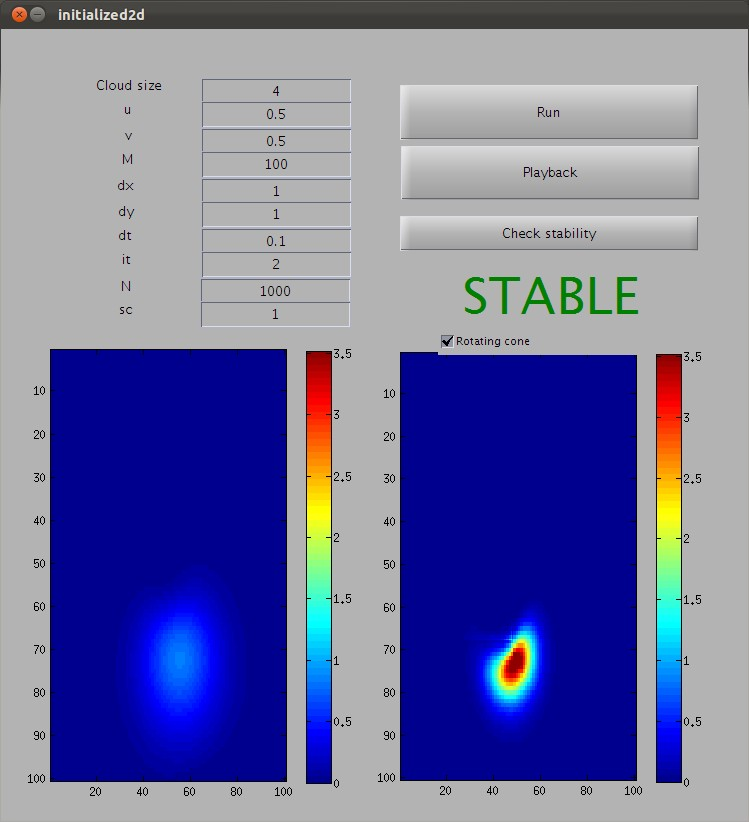
\includegraphics[width=0.5\textwidth]{matlabgui}
\end{figure}
\end{frame}


\subsection{Numerical Results}

\begin{frame}
\frametitle{Example of antidiffusion with an upstream scheme}
\begin{figure}
\renewcommand{\imsize}{0.7\textwidth}
\includegraphics<1>[width=\imsize]{animation/aanime0}%
\includegraphics<2>[width=\imsize]{animation/aanime1}%
\includegraphics<3>[width=\imsize]{animation/aanime2}%
\includegraphics<4>[width=\imsize]{animation/aanime3}%
\includegraphics<5>[width=\imsize]{animation/aanime4}%
\includegraphics<6>[width=\imsize]{animation/aanime5}%
\includegraphics<7>[width=\imsize]{animation/aanime6}%
\includegraphics<8>[width=\imsize]{animation/aanime7}%
\end{figure}
\end{frame}

\begin{frame}

\frametitle{Less diffusion}
Iterating with antidiffusion vector reduces diffusion.

\begin{figure}
\renewcommand{\imsize}{0.8\textwidth}
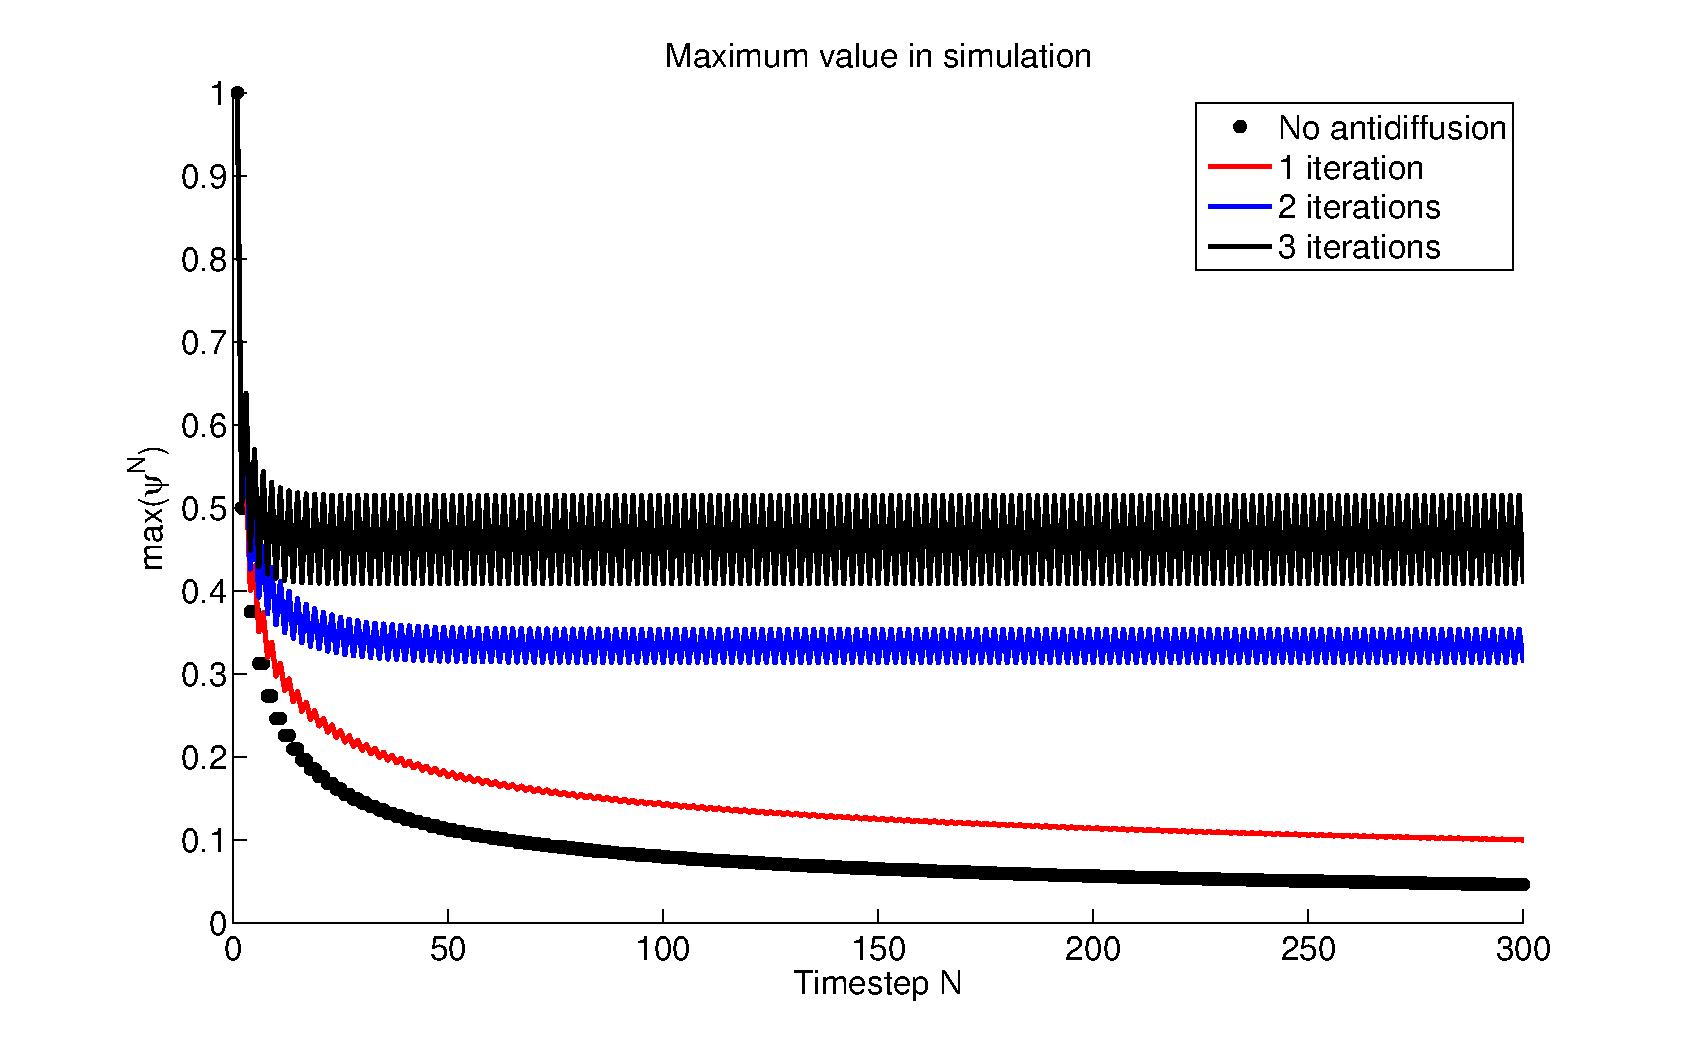
\includegraphics[width=\imsize]{maxs}%
\end{figure}
\end{frame}

\begin{frame}

\frametitle{Less interaction}
Simulations are more localized, less interaction between neighbouring pockets.

\begin{figure}
\renewcommand{\imsize}{0.9\textwidth}
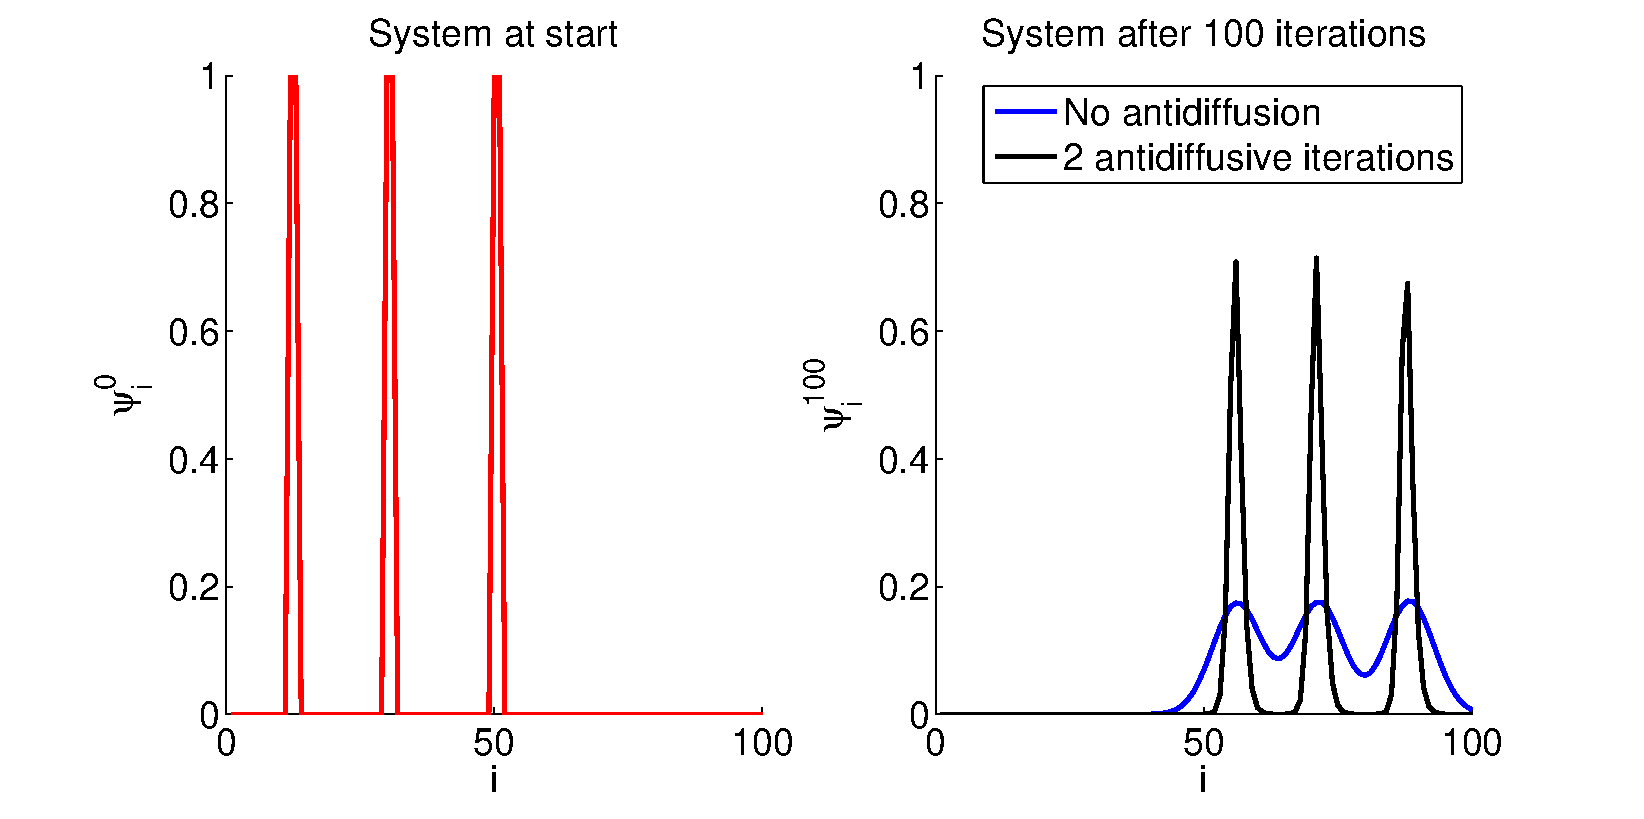
\includegraphics[width=\imsize]{animation/peaks}%
\end{figure}
\end{frame}

\begin{frame}
\frametitle{Example of diffusion with an upstream scheme}
Solid body rotation

\begin{figure}
\renewcommand{\imsize}{\textwidth}
\includegraphics<1>[width=\imsize]{animation2/anim-0}
\includegraphics<2>[width=\imsize]{animation2/anim-1}
\includegraphics<3>[width=\imsize]{animation2/anim-2}
\includegraphics<4>[width=\imsize]{animation2/anim-3}
\includegraphics<5>[width=\imsize]{animation2/anim-4}
\includegraphics<6>[width=\imsize]{animation2/anim-5}
\includegraphics<7>[width=\imsize]{animation2/anim-6}
\includegraphics<8>[width=\imsize]{animation2/anim-7}
\includegraphics<9>[width=\imsize]{animation2/anim-8}
\includegraphics<10>[width=\imsize]{animation2/anim-9}
\includegraphics<11>[width=\imsize]{animation2/anim-10}
\includegraphics<12>[width=\imsize]{animation2/anim-11}
\includegraphics<13>[width=\imsize]{animation2/anim-12}
\includegraphics<14>[width=\imsize]{animation2/anim-13}
\includegraphics<15>[width=\imsize]{animation2/anim-14}
\includegraphics<16>[width=\imsize]{animation2/anim-15}
\includegraphics<17>[width=\imsize]{animation2/anim-16}
\includegraphics<18>[width=\imsize]{animation2/anim-17}
\includegraphics<19>[width=\imsize]{animation2/anim-18}
\includegraphics<20>[width=\imsize]{animation2/anim-19}
\includegraphics<21>[width=\imsize]{animation2/anim-20}
\includegraphics<22>[width=\imsize]{animation2/anim-21}
\includegraphics<23>[width=\imsize]{animation2/anim-22}
\includegraphics<24>[width=\imsize]{animation2/anim-23}
\includegraphics<25>[width=\imsize]{animation2/anim-24}
\includegraphics<26>[width=\imsize]{animation2/anim-25}
\includegraphics<27>[width=\imsize]{animation2/anim-26}
\includegraphics<28>[width=\imsize]{animation2/anim-27}
\includegraphics<29>[width=\imsize]{animation2/anim-28}
\includegraphics<30>[width=\imsize]{animation2/anim-29}
\includegraphics<31>[width=\imsize]{animation2/anim-30}
\includegraphics<32>[width=\imsize]{animation2/anim-31}
\includegraphics<33>[width=\imsize]{animation2/anim-32}
\includegraphics<34>[width=\imsize]{animation2/anim-33}
\includegraphics<35>[width=\imsize]{animation2/anim-34}
\includegraphics<36>[width=\imsize]{animation2/anim-35}
\includegraphics<37>[width=\imsize]{animation2/anim-36}
\includegraphics<38>[width=\imsize]{animation2/anim-37}
\includegraphics<39>[width=\imsize]{animation2/anim-38}
\includegraphics<40>[width=\imsize]{animation2/anim-39}
\includegraphics<41>[width=\imsize]{animation2/anim-40}
\includegraphics<42>[width=\imsize]{animation2/anim-41}
\includegraphics<43>[width=\imsize]{animation2/anim-42}
\includegraphics<44>[width=\imsize]{animation2/anim-43}
\includegraphics<45>[width=\imsize]{animation2/anim-44}
\includegraphics<46>[width=\imsize]{animation2/anim-45}
\includegraphics<47>[width=\imsize]{animation2/anim-46}
\includegraphics<48>[width=\imsize]{animation2/anim-47}
\includegraphics<49>[width=\imsize]{animation2/anim-48}
\includegraphics<50>[width=\imsize]{animation2/anim-49}
\includegraphics<51>[width=\imsize]{animation2/anim-50}
\includegraphics<52>[width=\imsize]{animation2/anim-51}
\includegraphics<53>[width=\imsize]{animation2/anim-52}
\includegraphics<54>[width=\imsize]{animation2/anim-53}
\includegraphics<55>[width=\imsize]{animation2/anim-54}
\includegraphics<56>[width=\imsize]{animation2/anim-55}
\includegraphics<57>[width=\imsize]{animation2/anim-56}
\includegraphics<58>[width=\imsize]{animation2/anim-57}
\includegraphics<59>[width=\imsize]{animation2/anim-58}
\includegraphics<60>[width=\imsize]{animation2/anim-59}
\includegraphics<61>[width=\imsize]{animation2/anim-60}
\includegraphics<62>[width=\imsize]{animation2/anim-61}
\includegraphics<63>[width=\imsize]{animation2/anim-62}
\includegraphics<64>[width=\imsize]{animation2/anim-63}
\includegraphics<65>[width=\imsize]{animation2/anim-64}
\end{figure}
\end{frame}

\begin{frame}
\frametitle{Example of diffusion with an upstream scheme}
\begin{itemize}
\item Without antidiffusion, the body diffuses in one full rotation
\item With antidiffusion, the body keeps its shape
\end{itemize}
\end{frame}
%
% % All of the following is optional and typically not needed.
% \appendix
% \section<presentation>*{\appendixname}
% \subsection<presentation>*{For Further Reading}
%
% \begin{frame}[allowframebreaks]
%   \frametitle<presentation>{For Further Reading}
%
%   \begin{thebibliography}{10}
%
%   \beamertemplatebookbibitems
%   % Start with overview books.
%
%   \bibitem{Author1990}
%     A.~Author.
%     \newblock {\em Handbook of Everything}.
%     \newblock Some Press, 1990.
%
%
%   \beamertemplatearticlebibitems
%   % Followed by interesting articles. Keep the list short.
%
%   \bibitem{Someone2000}
%     S.~Someone.
%     \newblock On this and that.
%     \newblock {\em Journal of This and That}, 2(1):50--100,
%     2000.
%   \end{thebibliography}
% \end{frame}


\section{Current state of research}
\begin{frame}
\begin{itemize}
\item Since 1983 a lot of progress has been made
\item Advection calculations on the sphere pose new problems/possibilities
\item Finite difference as well as finite volume methods 
\item Faster machines, more complex schemes
\item Much higher accuracy
\item Improvements by Smolarkiewicz and others
\end{itemize}
\end{frame}

\begin{frame}
Reduced grid (Spee, 1991)
\begin{figure}
\renewcommand{\imsize}{0.75\textwidth}
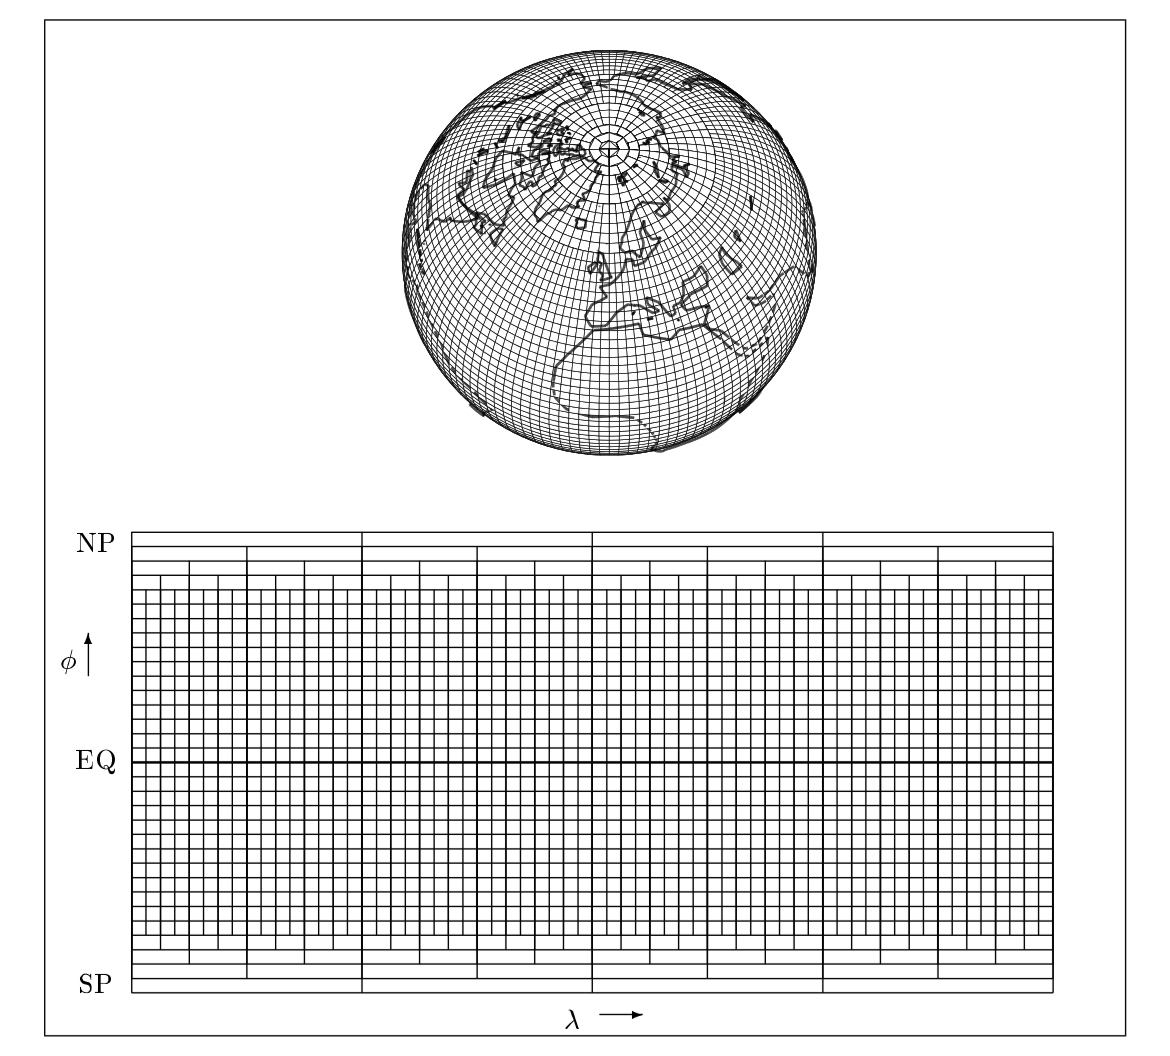
\includegraphics[width=\imsize]{globe}%
\end{figure}
\end{frame}

\begin{frame}
Spherical hexagonal-pentagonal grid (Lipscomb and Ringler, 2005) 
\begin{figure}
\renewcommand{\imsize}{0.75\textwidth}
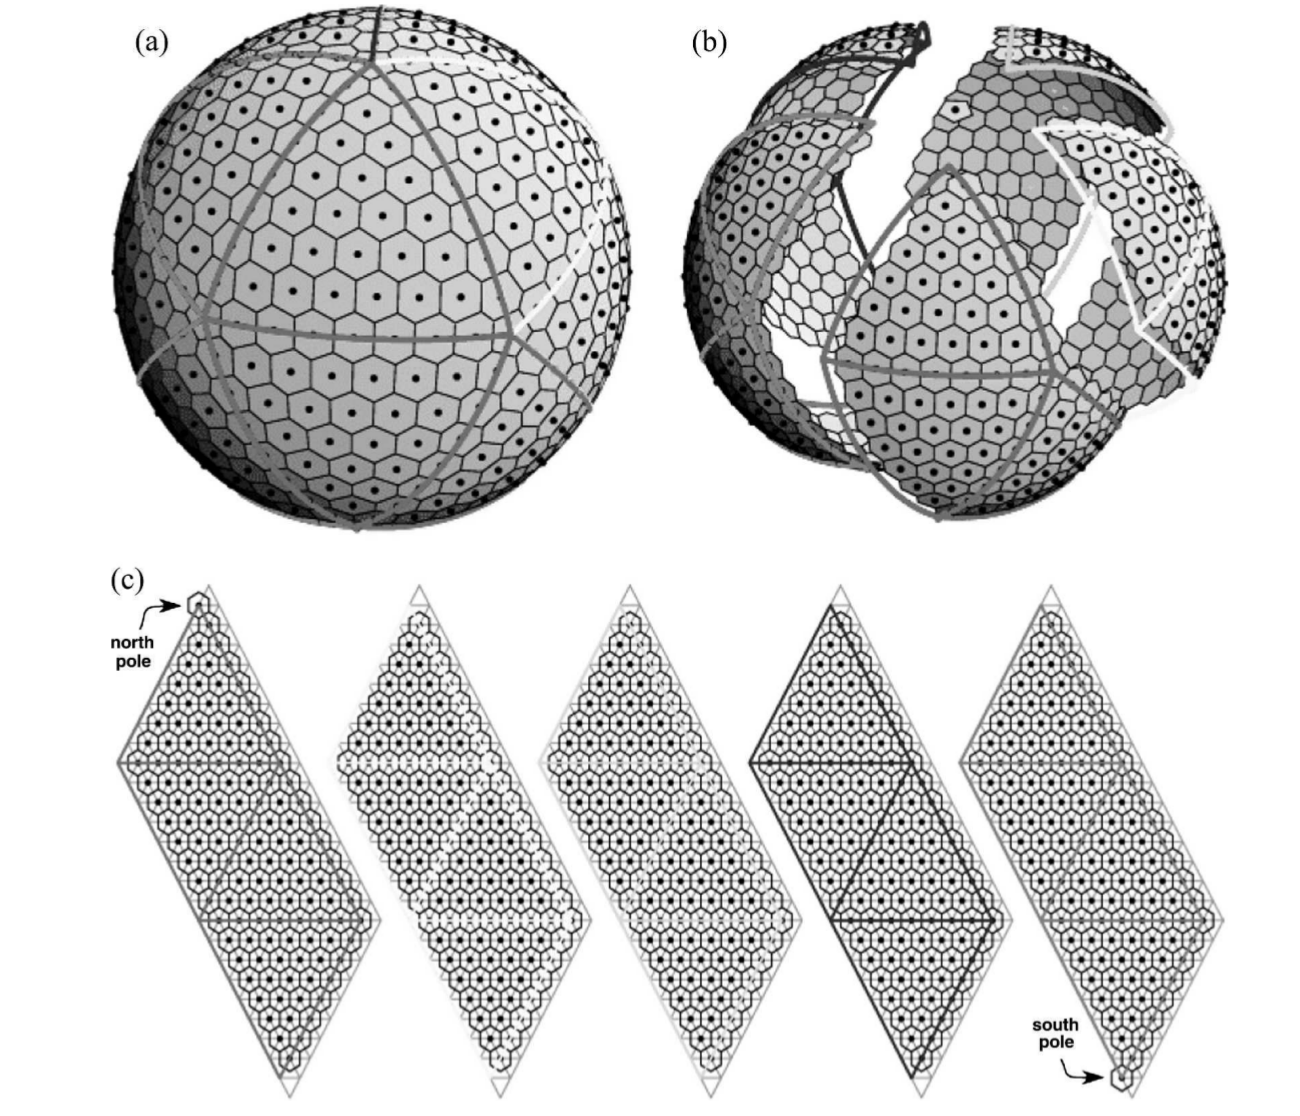
\includegraphics[width=\imsize]{lipcomb}%
\end{figure}
\end{frame}



\begin{frame}
\frametitle{MPDATA}

MPDATA: Multidimensional Positive Definite Advection Transport Algorithm

\begin{itemize}
\item Multidimensional generalization of Smolarkiewicz' original scheme
\item Widely used in finite difference form
\item Recently a transition to finite volume has been made
\end{itemize}

\begin{quotation}
Over the two decades, MPDATA evolved from an advection scheme into a class of generalized transport algorithms that expand beyond advective transport to alternate PDEs and complete fluid models with a wide range of underlying governing equations. 
\end{quotation} 
\begin{center}Smolarkiewicz, 2005\end{center}
\end{frame}

\section{Conclusions}
\begin{frame}
\begin{itemize}
\frametitle{Conclusions}
\item Diffusion is a threat for reliable advection simulations
\item Antidiffusive advection schemes reduce this threat and are thus important in SOAC
\item Smolarkiewicz' relatively simple scheme already significantly improves results
\end{itemize}

\begin{figure}
\renewcommand{\imsize}{0.75\textwidth}
\includegraphics<2>[width=\imsize]{thanks}%
\end{figure}
\end{frame}

\bibliographystyle{alpha}
\bibliography{presentation.bib}

\end{document}


